\cotefile{156-5}
\scanpage{42}\mspage{41}
c) L'\unsure{ens|ens.} des fermés pour ${\unsure{\mathcal{T}|\tau}}'$ est en corr. \unsure{biuniv.} avec l'\unsure{ens|ens.} des couples
\[
\begin{aligned}
(B,A_{\unsure{u|n|U}}) \qquad & B\unsure{\subset|\in}T\ \text{fermé pour }\mathcal{T}'_0\\
& A_u\ \text{fermé de }\unsure{U|u|n}=S\setminus T\ \text{pour }\mathcal{T}\mid(S\setminus T)
\end{aligned}
\]
\[
\text{tels que}\qquad \overline{A_u}\cap T\subset B \qquad
\text{(adh. prise pour }\mathcal{T}\text{)}\ \deleted{\unsure{\mathcal{T})}}.
\]

d) Si $\mathcal{T}'_0$ et $\mathcal{T}$ \unsure{ultra topologiques|ultratopologiques}, $\mathcal{T}'$ aussi\unsure{.} La relation de préordre associée \deleted{\unsure{se définit}} \inserted{se décrit} ainsi. Pour $x,y\in S$, on a $x\underset{\mathcal{T}'}{\leq}y$ sss
\[
\left\{\begin{aligned}
&\text{ou bien}\quad x,y\in T,\qquad x\underset{\mathcal{T}'}{\leq}y\\
&\left.\begin{aligned}
&\text{ou bien}\quad x,y\in U=S\setminus T,\qquad x\underset{\mathcal{T}}{\leq}y\\
&\text{ou bien}\quad x\in T,\ y\in U,\qquad x\underset{\mathcal{T}}{\leq}y
\end{aligned}\right]
\end{aligned}\right.
\]
\margin{en d'autres termes, si $y\in U$, on a $x\underset{\mathcal{T}'}{\leq}y$ sss \unsure{a} $x\underset{\mathcal{T}}{\leq}y$.}

e) \inserted{Sous les conditions de d)} Considérons les ens ordonnés $I,I'$ associés à $\mathcal{T},\mathcal{T}'$, et la partie \inserted{fermée} $J\subset I$ correspondant à la partie fermée $T$ de $(S,\mathcal{T})$, enfin l'application $\varphi:I'\unsure{\mathbin{\text{---}}|\longrightarrow}I$ canonique.
\diagram{\begin{tikzcd}[ampersand replacement=\&,column sep=small,row sep=large]
\varphi^{-1}(J)={} \& J' \arrow[d] \& \subset \& I' \arrow[d,"\varphi"] \& \overline{\mathcal{T}'} \arrow[d] \\
{} \& J \& \subset \& I \& \overline{\mathcal{T}}
\end{tikzcd}}

\deleted{Alors}, \deleted{\unsure{la|le}} Soit $\overline{\mathcal{T}'}$ \deleted{est} la \unsure{top|top.} de $\mathcal{T}'$ déduite de $\mathcal{T}'$ par passage au quotient \unsure{(ou encore,} associée à la relation \uline{d'ordre} sur $I'$ associé au préordre), $\widetilde{\mathcal{T}}$ la topologie sur $I'$ image inverse de $\overline{\mathcal{T}}$. Alors $\overline{\mathcal{T}'}$ est la moins fine des top. sur $I'$ qui \inserted{\unsure{sont plus fines que} $\widetilde{\mathcal{T}}$ et} induisent sur $J'$ la $\unsure{=}$ \deleted{\unsure{top}} topologie $\overline{\mathcal{T}}\mid J'$. Elle est
\scanpage{43}\mspage{42}
\uline{caractérisée} par les conditions suivantes :
% slanted
\margin{C'est faux, ça implique (i) (ii) (iii) (iv), mais ces conditions ne suffisent nullement, voir plus bas ! \unsure{p.|v.}~48}
\margin{i.e $\overline{{\unsure{\mathcal{T}|\tau}}'}\in\underline{\underline{\overline{\unsure{\mathscr{T}|\mathcal{T}}}}}$ $\left\{\vphantom{\rule{0pt}{4ex}}\right.$}

(i) $\overline{\mathcal{T}'}$ est plus fine que $\widetilde{\mathcal{T}}$, et induit sur $J'$ $\unsure{\widetilde{\mathcal{T}}|\overline{\mathcal{T}}}\mid J'$.

(ii) $\overline{\mathcal{T}'}\mid\overset{\deleted{\unsure{\sim|\mathord{-}}}}{{\unsure{U|u|n}}'}=I'\setminus J'$ coïncide avec $\widetilde{\mathcal{T}}\mid\overset{\deleted{\sim}}{U'}$

(iii) $\varphi\mid U'$ induit \deleted{\unsure{une bijection}} \inserted{\unsure{iso. préord.}} $U'\longrightarrow U=S\setminus T$
% slanted
\margin{\deleted{\unsure{Autant dire|Autrement dit}}}

(\unsure{iv|iiv}) La topologie de $I$ est quotient \unsure{final|finale|déduit} pour les applications $I'\unsure{\mathbin{\text{---}}|\longrightarrow}I$, $J\mathbin{\text{---}}I$ ($I'$ munie \deleted{\unsure{celle de} $I$, \unsure{conjointement}} \inserted{de $\overline{\mathcal{T}'}$, $J$ \deleted{\unsure{de}} muni de $\overline{\mathcal{T}}\mid J$}) (\unsure{Ce} qui exclut notamment la solution triviale pour (i) (ii), obtenue en prenant la topologie somme sur \deleted{\unsure{$J'$}} $I'=J'\underset{\text{disj.}}{\cup}\overset{\deleted{\sim}}{U'}$, sauf si $I$ lui\unsure{$=$} est une somme top. $J\sqcup\underset{\substack{\Vert\\I\setminus J}}{U}$).
% slanted
\margin{C'est cette condition que j'avais d'abord \unsure{oubliée|oublié}, à la page 31 !}
% slanted
\margin{\deleted{\unsure{Autant}} dire que $\mathcal{T}'$ sur $S$ est caractérisée par les propriétés analogues (i) (ii) (iii) (iv), la dernière \unsure{signifiant|signifie} que la top $\text{\textcircled{$\mathcal{T}$}}$ sur $S$ est finale pour $\unsure{\mathcal{T}''|\mathcal{T}'}$ sur $S$ et $\mathcal{T}$ sur $T$ (\unsure{id|et} $S\unsure{\rightrightarrows|\to}S$ $T\unsure{\hookrightarrow|\to}S$)}
% slanted
\margin{en fait, c'est indépendant \unsure{aussi|même} de l'hyp. \unsure{ultra-topologique}}

Démonstration

\deleted{\unsure{a) et b).}} \inserted{(a b c)} Il est clair que les ens. \unsure{épinglés} dans c) sont ceux qui satisfont $1^\circ)$, $2^\circ)$ $3^\circ)$ dans b), et que la représentation dans c) est unique. Il reste à voir, pour prouver (a,b,c), que les ens. forment une topologie, \deleted{et} qu'elle \deleted{\unsure{a les propriétés}} \inserted{est} dans $\underline{\mathcal{T}}$, et est moins fine des top $\in\underline{\mathcal{T}}$.

1) Ce sont les fermés d'une topologie.

Stables par intersections quelconques : clair

Stables par réunions finies : idem.

C'est \unsure{$=$} stable par réunions \unsure{quelconques} s'il en est ainsi \unsure{pour|dans} $(T,\mathcal{T}'_0)$, $(\deleted{\unsure{D|I}}\unsure{S|I},\mathcal{T})$, d'où la première assertion de \unsure{d)|a)}.

\scanpage{44}\mspage{43}
Cette topologie est plus fine que $\unsure{\mathcal{T}|\tau}\deleted{\unsure{'}}$, i.e. si $X$ est fermé dans $\mathcal{T}$, il \unsure{satisfait|satisfont} ces conditions : clair. Il induit $\mathcal{T}'_0$, i.e. si $X\subset T$, il satisfait ces cond. sss il est fermé pour $\mathcal{T}'_0$ : clair. Donc $\mathcal{T}'\in\underline{\unsure{\mathscr{T}|\mathcal{T}}}$. Prouvons que c'est un plus grand élément (top la moins fine). i.e que pour \deleted{\unsure{tout}} $\mathcal{T}''\in\underline{\mathcal{T}}$, les fermés pour $\mathcal{T}'$ sont des fermés pour $\mathcal{T}''$. En effet, on a
\[
X=B\deleted{\unsure{\cap}}\cup\overline{X\cap\unsure{U|u|n}}^{(\mathcal{T})}
\]
$B$ étant fermé dans $T$. (pour $\mathcal{T}'_0$\inserted{\deleted{\unsure{donc pour}} $\mathcal{T}^{\prime\prime\unsure{,}}\mid\overset{\unsure{\sim|\text{ou}}}{T}$}), et $T$ étant \uline{fermé} dans $\deleted{\unsure{T}}S$ pour $\mathcal{T}$ donc \inserted{a fortiori} pour $\mathcal{T}''$, $B$ est fermé dans $S$ pour $\mathcal{T}''$.
% slanted
\margin{(C'est la première fois qu'on utilise $T$ fermé dans $S$}
De $\unsure{=}$ $\overline{X\cap U}^{(\mathcal{T})}$ étant fermé pour $\mathcal{T}$, l'est pour $\unsure{:}\mathcal{T}''$, donc $X=B\cup\overline{X\cap U}^{(\mathcal{T})}$ l'est aussi\unsure{.} Cela prouve a) b) c).

Prouvons d)\inserted{(le début déjà prouvé)}, en nous rappelant que pour $x,y\in T$,
\[
\begin{aligned}
x\underset{\mathcal{T}'}{\leq}y&\Longleftrightarrow\overline{x}^{(\mathcal{T}')}\subset\overline{y}^{(\mathcal{T}')}\\
&\Longleftrightarrow x\in\overline{y}^{(\mathcal{T}')}.
\end{aligned}
\]
Comme $\mathcal{T}'\mid U\unsure{\ne|=}\mathcal{T}\mid U$, et $\mathcal{T}'\mid T=\mathcal{T}'_0$, les cas $x,y\in T$ et $x\unsure{,}y\in U$ sont déjà clairs. Reste \unsure{le|les} cas où soit $x\in U,y\in T$, soit l'inverse. Le premier cas ne peut se produire, car si $y\in T$, $\overline{y}^{(\mathcal{T}')}\unsure{\in|\subset}T$ ($T$ \uline{fermé} dans $S$ pour $\mathcal{T}'$) donc $x\notin\overline{y}^{(\mathcal{T}')}$ \deleted{puisque} si $x\in U$. Donc reste le cas $[x\in T,]$ $y\in U$, prouver $x\underset{\mathcal{T}'}{\leq}y\Longleftrightarrow x\underset{\unsure{\mathcal{T}'|\mathcal{T}}}{\leq}y$
\margin{NB c'est vrai sans supposer $x\in\unsure{T|S}$}
\scanpage{45}\mspage{44}
donc il faut voir que l'adhérence de $y$ pour ${\unsure{\mathcal{T}|\tau}}'$, et pour $\mathcal{T}$, est pareille (a priori la première serait plus petite). \deleted{Soit en effet $X$ un fermé de $X$, tel que} \inserted{\unsure{Explicitons} en fait}

\uline{Corollaire} Sous \deleted{\unsure{$X$ est une}} \unsure{les|ces} conditions de a) b) c) (sans se restreindre au cas des ultratopologies) si $\unsure{X|A}$ est une partie de $\unsure{U|u|n}$, son adhérence pour $\mathcal{T}'$, et pour $\mathcal{T}$, est la \unsure{$=$}. \deleted{(Idem bien sûr pour une partie de $T$.)}
% slanted
\margin{Cela donne l'adhérence d'une partie quelconque $\deleted{\unsure{X|A}}$ de $S$, pour $\mathcal{T}'$, en termes de $\mathcal{T}$ et de $\mathcal{T}'_0$, \unsure{comme|car} \deleted{$\unsure{\bar{X}^{(\mathcal{T}')}}$}
\[
\bar{X}^{(\mathcal{T}')}=\left(\overline{X\cap U}^{(\mathcal{T})}\right)\cup\overline{(X\cap T)}^{(\mathcal{T}'_0)}
\]}

Soit en effet $X\supset A$, fermé pour $\unsure{T'|\mathcal{T}'}$. alors par les conditions $1^\circ,2^\circ,3^\circ)$ plus haut, $X\supset\overline{X\cap U}^{(\mathcal{T})}$, donc si $X\supset A$, $X\supset\overline{A}^{(\mathcal{T})}$, \deleted{\unsure{a fortiori}} en particulier $\overline{A}^{(\mathcal{T}')}\supset\overline{A}^{(\mathcal{T})}$, OK.

Prouvons e). La première assertion (bas de la page) est une simple \unsure{fonctorialité|formalité|fontorialité}, qui devrait être évidente. \inserted{Les conditions (i) (ii) (iii) pour $\mathcal{T}'$ sont \unsure{dès lors|alors|déjà} connues.} Montrons que la top. de $I$ est \deleted{\unsure{quotient de celle de} $I'$, \unsure{donc}} \inserted{finale pour $J\unsure{\mathbin{\text{---}}|\longrightarrow}I$, $I'\longrightarrow I$.} Cela signifie que pour une partie de $I'$ qui est \uline{$\widetilde{\mathcal{T}}$-saturée} (i.e. de la forme $\varphi^{-1}(A)$), celle-ci est fermée pour $\widetilde{\mathcal{T}}$ si (et seulem\textsuperscript{t} si) elle l'est pour $\overline{\mathcal{T}'}$, \uuline{et} sa trace sur $J'$ est fermée pour $\overline{\mathcal{T}}$. Cela revient à ceci, \deleted{\unsure{une}}
\scanpage{46}\mspage{45}
en revenant \deleted{\unsure{à|au}} à la situation initiale

\uline{Corollaire} \deleted{Dans le cas des ultratopologies, \unsure{une}} \inserted{(Vaut sans se restreindre aux ultratopologies) Soit} \deleted{\unsure{fer}} $A$ une partie de $T$ \deleted{[saturée pour $\unsure{\mathcal{T}|\tau}$.]} Pour qu'elle soit fermée \uline{pour $\mathcal{T}$}, il f et s qu'elle \deleted{\unsure{le}} soit a) fermée \uline{pour $\mathcal{T}'$} et b) sa trace sur $T$ soit fermée \uline{pour $\mathcal{T}$}.
% slanted
\margin{saturation inutile,}
\margin{i.e. la top. $\mathcal{T}$ sur $S$ est finale pour \diagram{\begin{tikzcd}[ampersand replacement=\&,row sep=tiny,column sep=small]
S \arrow[r,"\mathrm{id}"] \& S\\
T \arrow[r,"{\text{\unsure{inc.|incl.}}}"] \& S
\end{tikzcd}} \unsure{pour} \deleted{\unsure{les}} les topologies \[\begin{aligned}&\mathcal{T}'\text{ sur } S,\\&\mathcal{T}\mid T\text{ sur }T\end{aligned}\]}

\deleted{C'est évidemment nécessaire. \unsure{Prouvons|Voyons} que c'est suffisant, \deleted{\unsure{a. Comme}} Comme $X$ est fermé pour $\mathcal{T}'$, \deleted{\unsure{donc}} on a (d'après \textcircled{b}) que $X\cap\unsure{U|u|n}$ \inserted{$=X_{\unsure{u|n|U}}$} est fermé pour $\mathcal{T}\mid U$, \inserted{d'où $\overline{X_u}^{(\mathcal{T})}\unsure{\subset|=}X_u$.} et que $\overline{\deleted{\unsure{A|B}}X_u}^{(\mathcal{T})}\deleted{\unsure{\in}}\cap T\subset X_B$, Comme $X_B$ est fermé dans $T$ \unsure{pour} $\mathcal{T}$ par hypothèse, \inserted{et $X=\overline{X_u}^{\mathcal{T}}\cup X_B$} il s'ensuit que $X$\unsure{-}}

Se voit aussitôt sur la formule
\[
\overline{X}^{(\mathcal{T}')}=\overline{X\cap U}^{(\mathcal{T})}\cup\overline{X\cap T}^{(\mathcal{T}'_0)}
\]
(page 44, marge), si $X$ est fermée pour $\mathcal{T}'$ on a
\[
\begin{aligned}
X&=\text{second membre}\ \deleted{\unsure{{}=X}},\quad\text{donc}\\
&=\overline{X\cap U}^{(\mathcal{T})}\cup
\underbrace{(X\cap T)}_{\substack{\text{car }X\cap T\text{ fermé}\\\text{pour }\mathcal{T},\text{ a fortiori}\\\text{pour }\mathcal{T}'_0}}
\qquad\text{donc}
\end{aligned}
\]
\deleted{\unsure{fer}} fermé comme réunion de deux fermés.

\scanpage{47}\mspage{46}
\margin{\figure{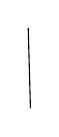
\begin{tikzpicture}[x=1pt,y=1pt]\draw (0,0) -- (.8,-29);\end{tikzpicture}}}
\uline{Corollaire} \inserted{(Cas ultratopologique)} Supposons que la top. de $J'$ soit quotient de celle de $J$, \deleted{Alors} i.e. $\varphi^{\unsure{*|\star}}:J'\longrightarrow \deleted{\unsure{I}}J$ submersif. Alors $\varphi$ aussi.

\uline{Corollaire} \inserted{(\unsure{Ultratopologies})} Supposons $\varphi^*$ submersif \unsure{à|;} fibres $0$-connexes -- alors $\varphi$ \unsure{item|idem|itou}. Supposons $\varphi^*$ \deleted{\unsure{aussi}} homotopiquement propre i.e. les $\varphi^{{*\unsure{)|\prime}}^{-1}}(J_{\deleted{\unsure{<|\leq}}\unsure{\leq|<}x})$ ``faiblement contractiles''. \deleted{\unsure{(quasi-hom}} Alors kif-kif pour $\varphi\deleted{^{\unsure{*|\leq}}}$.

On est ramené à prouver que si $I$ admet un plus grand élément \inserted{$x$} (donc est f.c.)\inserted{$x\notin J$}, alors $I'$ est f. \unsure{kontractile|contractile}. Mais considérons l'unique élément \inserted{$x'$} de $I'$ au dessus de $x$, prouvons que c'est un plus grand élément. En effet, comme $x'\in I'\setminus{\unsure{U|u|n}}'$, son adhérence \unsure{pour} $\overline{{\unsure{\mathcal{T}|\tau}}'}$, et pour $\unsure{\overline{\mathcal{T}}|\widetilde{\mathcal{T}}}$, est la \unsure{$=$}, donc c'est tout. OK !

\uline{Corollaire} \inserted{(Ultratopologies)} Si $\varphi^*$ est homotopiquement propre à fibres \deleted{\unsure{fib}} faiblement contractibles (donc une équivalence d'homotopie faible universelle), \unsure{item|idem} pour $\varphi$.

\scanpage{48}\mspage{47}
Mais je n'ai pas \unsure{terminé} \unsure{entièrement} : prouver e), il faut montrer que ${\unsure{\mathcal{T}|\tau}}'$ \inserted{(ou $\overline{\mathcal{T}'}$)} est \uline{caractérisée} par les conditions dites.
% slanted
\margin{\unsure{mais|Mais} c'est faux !!}

Donc il faut voir que si $\mathcal{T}''$ sur $\deleted{\unsure{I}}S$ satisfait les conditions
\[
\left\{\begin{aligned}
&\text{(i)}\quad\mathcal{T}''\leq\mathcal{T}\\
&\text{(ii)}\quad\mathcal{T}''\mid T=\mathcal{T}'_0\\
&\text{(iii)}\quad\mathcal{T}''\mid\unsure{U|u|n}=\mathcal{T}\mid U\qquad (U=\unsure{T|\mathcal{T}}\setminus S)\\
&\text{(iv)}\quad\text{Toute partie \deleted{de} }X\text{ de }S\ \text{\deleted{\unsure{telle}} qui est}\\
&\qquad\text{fermée pour }\mathcal{T}''\text{ et telle que }X\cap T\text{ fermée}\\
&\qquad\text{pour }\mathcal{T},\ \text{est fermé pour }\mathcal{T},
\end{aligned}\right.
\]
% slanted
\margin{i.e. top. $\mathcal{T}$ est finale pour
\diagram{\begin{tikzcd}[ampersand replacement=\&,column sep=small,row sep=small]
\underset{(\mathcal{T}'')}{S}\arrow[r,"\mathrm{id}"] \& S\\
\underset{(\mathcal{T})}{T}\arrow[ur,hook,"\unsure{\mathrm{in}|\mathrm{inj}}"']
\end{tikzcd}}}
alors $\mathcal{T}''=\mathcal{T}'$. On sait déjà, \unsure{en raison de} (i) (ii), que $\mathcal{T}''\leq\mathcal{T}'$, reste à voir l'inverse, i.e. que tt fermé pour $\mathcal{T}''$ est fermé pour $\mathcal{T}'$, donc satisfait les conditions $1^\circ$ $2^\circ$ $3^\circ$ de \deleted{\unsure{Or si} $X$ fermé pour $\mathcal{T}''$,} \textcircled{b}.

\[
\begin{aligned}
1^\circ)&\quad X\cap U\ \text{est fermé dans }U\ \text{pour }\mathcal{T}\mid U\\
&\qquad\text{OK puisque }\mathcal{T}''\mid U=\mathcal{T}\mid U\quad\text{(iii)}
\end{aligned}
\]

\[
\begin{aligned}
2^\circ)&\quad X\cap T\ \text{fermé dans }T\ \text{pour }\mathcal{T}'_0\\
&\qquad\text{OK \unsure{puis|par|puisque} }\mathcal{T}''\mid T=\mathcal{T}'_0\quad\text{(ii)}
\end{aligned}
\]

\[
3^\circ)\quad\overline{X_{\unsure{u|n|U}}}^{(\mathcal{T})}\cap T\subset X\deleted{_{\unsure{B|T}}}\cap T
\]
C'est ici sans doute qu'il faut utiliser (iv). Il faudrait prouver qu'on a
\[
\overline{X_u}^{(\mathcal{T})}\underset{\text{donc }=}{\subset}\overline{X_u}^{(\mathcal{T}'')}
\quad\bigl(\subset\overline{X}^{(\mathcal{T}'')}\bigr)
\underset{\substack{\text{car }X\\\text{fermé pour }\mathcal{T}''}}{=}X
\]
et \unsure{ça|sa} donnerait ce qu'on \unsure{veut}.

Donc il faudrait prouver que pour $A\subset U$,
\[
\overline{A}^{(\mathcal{T}'')}=\overline{A}^{(\mathcal{T})},\ \text{i.e.}\quad
\text{\uuline{$\overline{A}^{(\mathcal{T}'')}$ est $\mathcal{T}$-fermé}}
\]
\scanpage{49}
\mspage{48}
et par la condition (iv), il reste à vérifier que
\[
\overline{A}^{({\unsure{\mathcal{T}|\tau}}'')}\cap T\quad\text{est}\quad\mathcal{T}\text{ fermée}\quad ??
\]
% slanted
\margin{C'est peut-être faux ?}

C'est ultra faux \unsure{on voit|en voici|on va voir}

\diagram{\begin{tikzcd}[ampersand replacement=\&,column sep=2.05em,row sep=.75em,
execute at end picture={
\draw ([xshift=-9pt,yshift=5pt]u.center) .. controls ([xshift=-9pt,yshift=19pt]u.center) and ([xshift=4pt,yshift=30pt]u.center) .. ([xshift=20pt,yshift=31pt]u.center) .. controls ([xshift=10pt,yshift=32pt]b.center) and ([xshift=24pt,yshift=18pt]b.center) .. ([xshift=26pt,yshift=6pt]b.center) .. controls ([xshift=23pt,yshift=-13pt]b.center) and ([xshift=10pt,yshift=-12pt]b.center) .. ([xshift=-11pt,yshift=-12pt]b.center) .. controls ([xshift=-6pt,yshift=-12pt]a.center) and ([xshift=-17pt,yshift=-11pt]a.center) .. ([xshift=-18pt,yshift=-2pt]a.center) .. controls ([xshift=-18pt,yshift=1pt]u.center) and ([xshift=-11pt,yshift=3pt]u.center) .. cycle;
\draw ([xshift=-17pt,yshift=10pt]j.center) .. controls ([xshift=-8pt,yshift=12pt]j.center) and ([xshift=14pt,yshift=12pt]q.center) .. ([xshift=20pt,yshift=9pt]q.center) .. controls ([xshift=35pt,yshift=-10pt]q.center) and ([xshift=18pt,yshift=-24pt]q.center) .. ([xshift=-3pt,yshift=-28pt]q.center) .. controls ([xshift=-20pt,yshift=-34pt]j.center) and ([xshift=-27pt,yshift=-22pt]j.center) .. ([xshift=-26pt,yshift=-7pt]j.center) .. controls ([xshift=-26pt,yshift=0pt]j.center) and ([xshift=-24pt,yshift=6pt]j.center) .. ([xshift=-23pt,yshift=8pt]j.center);
\path (u.center) -- (b.center) coordinate[pos=.27](hA) coordinate[pos=.34](hB) coordinate[pos=.41](hC) coordinate[pos=.48](hD) coordinate[pos=.55](hE) coordinate[pos=.62](hF) coordinate[pos=.69](hG);
\foreach \p in {hA,hB,hC,hD,hE,hF,hG}{\draw[line width=.65pt] ([xshift=-2.3pt,yshift=-2pt]\p) -- ([xshift=2.3pt,yshift=2pt]\p);}
\path (u.center) -- (b.center) node[midway,yshift=19pt] {$\overbrace{\rule{2em}{0pt}}^{I'}$};
\path (j.center) -- (q.center) node[midway,yshift=-14pt] {$\underbrace{\rule{2em}{0pt}}_{I}$};
\path (u.center) -- (a.center) node[midway,xshift=-22pt] {$\deleted{\unsure{J'|J}}\deleted{\Bigl\{ }$};
\node at ([xshift=-18pt,yshift=-9pt]j.center) {$J$};
\draw[->,line width=.8pt] ([xshift=-12pt,yshift=-7pt]j.center) -- ([xshift=-5pt,yshift=-3pt]j.center);
\draw[->] ([xshift=37pt,yshift=14pt]b.center) -- node[right] {$\varphi$} ([xshift=37pt,yshift=1pt]q.center);
\node at ([xshift=30pt,yshift=-3pt]q.center) {$\deleted{\unsure{I|J}}$};
}]
|[alias=u]| \bullet \arrow[dr] \& {}\\
|[alias=a,label=left:{\(a\)}]| \bullet \arrow[r] \& |[alias=b,label=right:{\(b\)}]| \bullet\\[1.7em]
|[alias=j]| \bullet \arrow[r] \& |[alias=q]| \bullet
\end{tikzcd}}

$I'$ a trois éléments, $I$ en \unsure{a} deux, $J$ un seul, $J'$ deux. On prend $A=\{b\}$, son adhérence pour $\mathcal{T}$ est $I'$ \unsure{tout|\deleted{tout}} entier, pour $\mathcal{T}'$ c'est $\{a,b\}$.

\figure{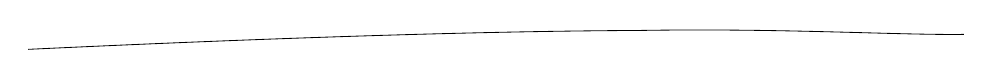
\begin{tikzpicture}[x=\linewidth,y=1mm]
\draw[line width=.3pt] (0,0) .. controls (.21,1.2) and (.45,2.3) .. (.64,2.4) .. controls (.79,2.7) and (.91,1.8) .. (.98,1.9);
\end{tikzpicture}}
\margin{\figure{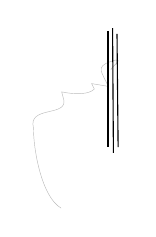
\begin{tikzpicture}[x=1pt,y=1pt]
\draw[black!27,line width=.16pt] (-17,-64) .. controls (-24,-60) and (-27,-43) .. (-27,-35) .. controls (-29,-27) and (-15,-31) .. (-16,-25) -- (-16.8,-22) .. controls (-12,-23) and (-7,-23) .. (-5,-21) -- (-6,-19) -- (0,-20) .. controls (-2,-15) and (-5,-13) .. (1,-11) .. controls (7,-9) and (1,-13) .. (1,-14);
\draw[line width=.65pt] (0,0) -- (0,-42);
\draw (1.6,1) -- (1.9,-44);
\draw (3.2,-1) -- (3.6,-42);
\end{tikzpicture}}}
Finalement, la condition \unsure{irréductible} à imposer à $\mathcal{T}'$ pour la caractériser dans $\underline{\underline{\mathcal{T}}}$, c'est la condition évidente : pour $A\subset \unsure{U|u|n}=S\setminus T$, son adhérence pour $\mathcal{T}$, et pour $\mathcal{T}'$, est la $=$ (ce qui implique déjà $\mathcal{T}\mid U=\mathcal{T}'\mid U$)

Cela donne l'adhérence d'une partie quelconque $A$, comme
\[
\overline{A}^{(\mathcal{T}')}=\overline{A\cap U}^{(\mathcal{T})}\cap\overline{(A\cap T)}^{(\mathcal{T}'_0)}
\]

